\documentclass{beamer}
\usetheme{Boadilla}
\usepackage{amsmath,amssymb,amsthm,latexsym,enumerate}
\usepackage{caption}
\usepackage{subcaption}
\usepackage{curves}
\usepackage{color}
\usepackage{epic}
\usepackage{tikz}
\usetikzlibrary{automata, positioning}
\graphicspath{{./images/}}
\usepackage{siunitx}

\title{Dissertation Presentation}
\subtitle{Hidden Markov Models for Rainfall Simulation}
\author{183773}
\institute{University of Sussex}
\date{Spring 2021}


\begin{document}

    \begin{frame}
        \titlepage
    \end{frame}

    \begin{frame}
        \frametitle{Outline}
        \tableofcontents
    \end{frame}

    \section{Hidden Markov Models}
    \begin{frame}
        \frametitle{Hidden Markov Models}
        \centering
        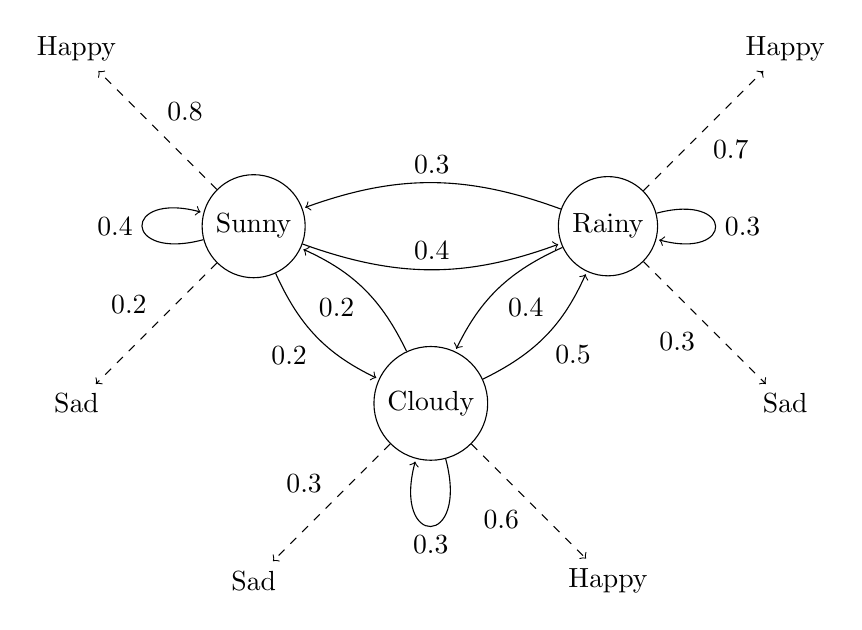
\begin{tikzpicture}[scale=0.75]
            \node[state] at(-3,0) (s) {Sunny};
            \node[state] at(3,0)  (r) {Rainy};
            \node[state] at(0,-3)  (c) {Cloudy};
            \node at (-6,3) (h1) {Happy};
            \node at (-6,-3) (s1) {Sad};
            \node at (3,-6) (h2) {Happy};
            \node at (-3,-6) (s2) {Sad};
            \node at (6,3) (h3) {Happy};
            \node at (6,-3) (s3) {Sad};

            \draw[every loop]
                (s) edge[bend right=20, auto=left] node {0.4} (r)
                (s) edge[bend right=20, auto=right] node {0.2} (c)
                (s) edge[loop left] node {0.4} (s)       
                (r) edge[bend right=20, auto=left] node {0.4} (c)
                (r) edge[bend right=20, auto=right] node {0.3} (s)
                (r) edge[loop right] node {0.3} (r) 
                (c) edge[bend right=20, auto=right] node {0.5} (r)
                (c) edge[bend right=20, auto=left] node {0.2} (s)
                (c) edge[loop below] node {0.3} (c);

            \draw [->, dashed] (s) edge[auto=right] node{0.2} (s1);
            \draw [->, dashed] (s) edge[auto=right] node{0.8} (h1);
            \draw [->, dashed] (c) edge[auto=right] node{0.3} (s2);
            \draw [->, dashed] (c) edge[auto=right] node{0.6} (h2);
            \draw [->, dashed] (r) edge[auto=right] node{0.3} (s3);
            \draw [->, dashed] (r) edge[auto=right] node{0.7} (h3);
        \end{tikzpicture}
    \end{frame}

    \section{Rainfall Models}
    \begin{frame}
    \frametitle{Rainfall Models}
        \begin{columns}
            \column{0.25\textwidth}
            Using Grando's model and fitting methodology, we run multiple attempts on estimating parameter $\tau_3$ but find different estimates.

            The uniform scatter is for the adjusted algorithm.
            \column{0.75\textwidth}
            \centering
            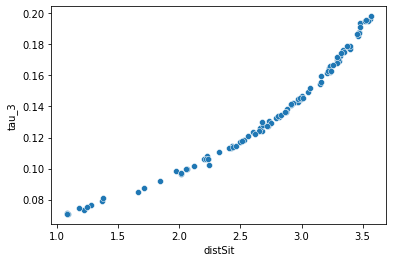
\includegraphics[width=0.3\linewidth]{./SingleParam/tau_3_1.png}
            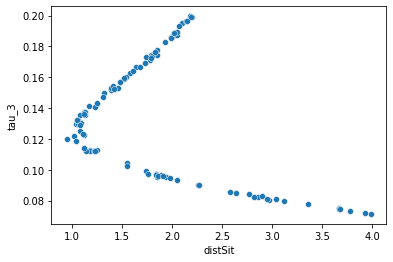
\includegraphics[width=0.3\linewidth]{./SingleParam/tau_3_2.png}
            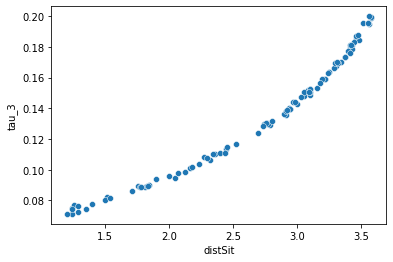
\includegraphics[width=0.3\linewidth]{./SingleParam/tau_3_3.png}
            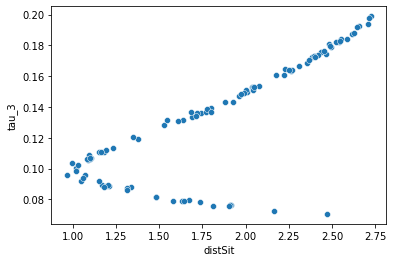
\includegraphics[width=0.3\linewidth]{./SingleParam/tau_3_4.png}
            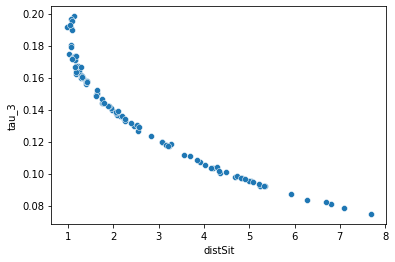
\includegraphics[width=0.3\linewidth]{./SingleParam/tau_3_5.png}

            
            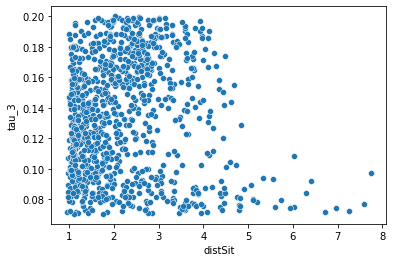
\includegraphics[width=0.3\linewidth]{./Adj_ABC/tau_3.png}
            
            \scriptsize{distSit = normalised Euclidean Distance between sample and simulation}
        \end{columns}
    \end{frame}
    
    \section{Simple Rainfall HMM}
    \begin{frame}
        \frametitle{Simple Rainfall HMM}
        \begin{columns}
            \column{0.5\textwidth}
            Sample(Top) vs Simulated(Bottom) data Frequencies
            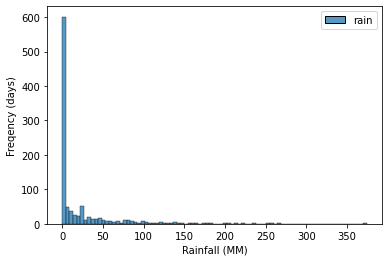
\includegraphics[width=0.8\linewidth]{HMM_Only/0_freq_data.png}
            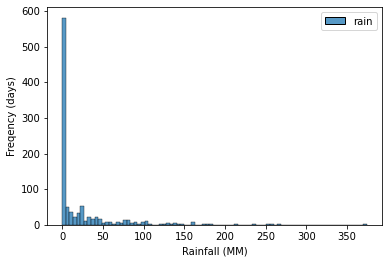
\includegraphics[width=0.8\linewidth]{HMM_Only/0_freq_sim.png}
            \column{0.5\textwidth}
            Sample(Top) vs Simulated(Bottom) data Frequencies not including 0mm days
            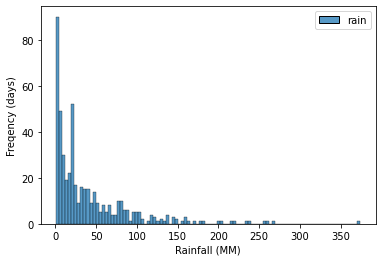
\includegraphics[width=0.8\linewidth]{HMM_Only/_freq_data.png}
            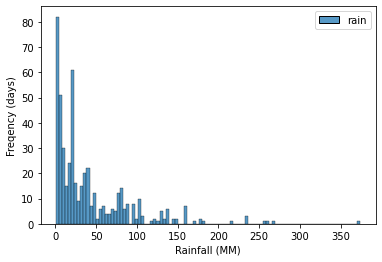
\includegraphics[width=0.8\linewidth]{HMM_Only/_freq_sim.png}
        \end{columns}
    \end{frame}

    \section{Generalised Model}
    \begin{frame}
        \frametitle{Generalised Model}
        \begin{columns}
            \column{0.2\textwidth}
            First row
            $\lambda \in [0,10]$ $\tau \in [0,10]$
            Second Row
            $\lambda \in [0,2]$ $\tau\in [0,0.5]$
            Third Row
            $\lambda\in [0.5,0.75]$ $\tau\in [0,0.1]$
            \column{0.8\textwidth}
            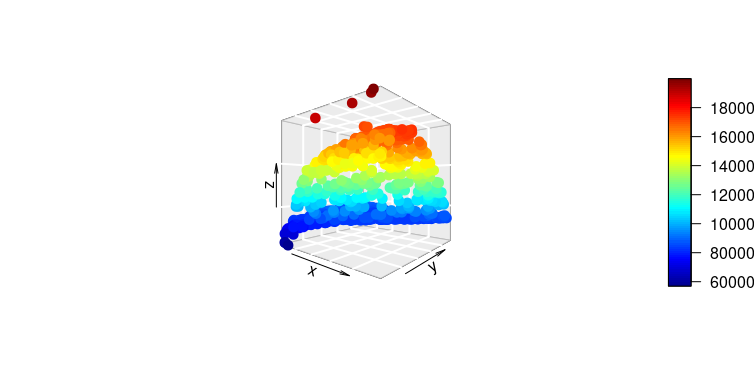
\includegraphics[width=0.3\linewidth]{Parameter Estimation on Attempt _1/param_1/lam0-10tau0-10.png}
            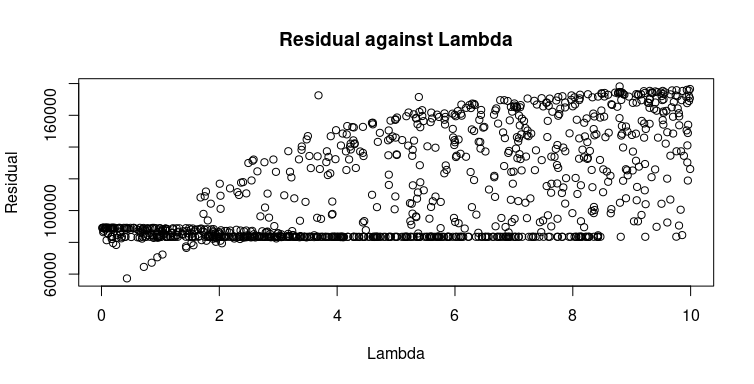
\includegraphics[width=0.3\linewidth]{Parameter Estimation on Attempt _1/param_1/lam_1.png}
            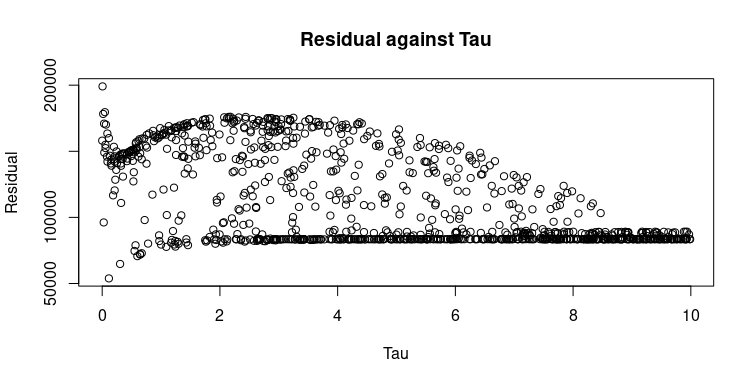
\includegraphics[width=0.3\linewidth]{Parameter Estimation on Attempt _1/param_1/tau_1.png}
    
            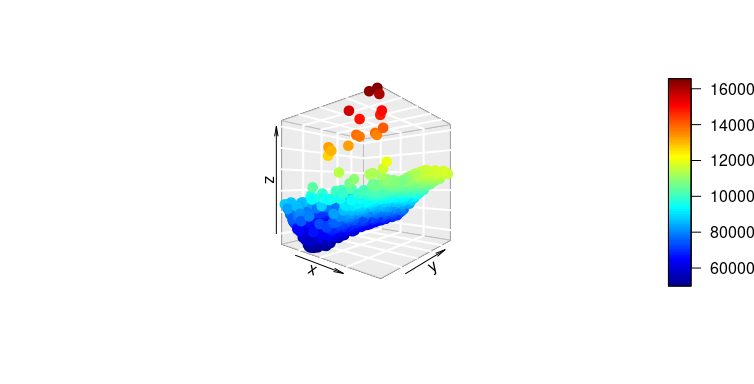
\includegraphics[width=0.3\linewidth]{Parameter Estimation on Attempt _1/param_1/lam0-2tau0-0_5.png}
            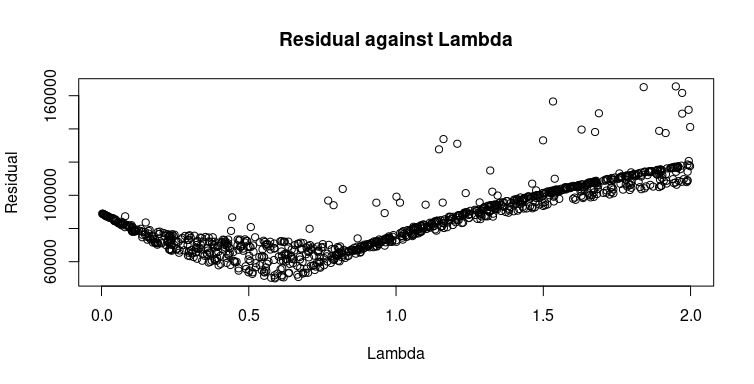
\includegraphics[width=0.3\linewidth]{Parameter Estimation on Attempt _1/param_1/lam_2.png}
            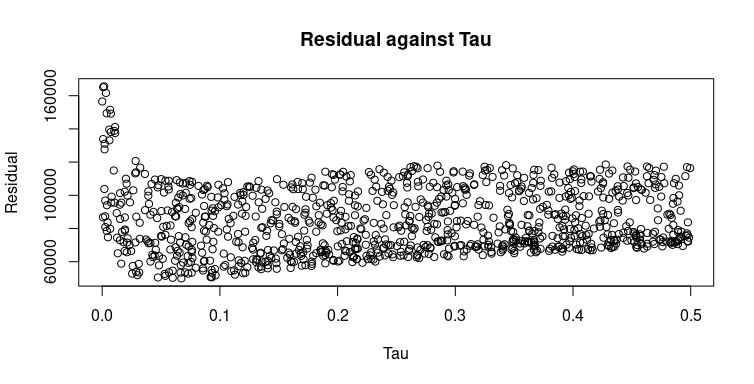
\includegraphics[width=0.3\linewidth]{Parameter Estimation on Attempt _1/param_1/tau_2.png}

            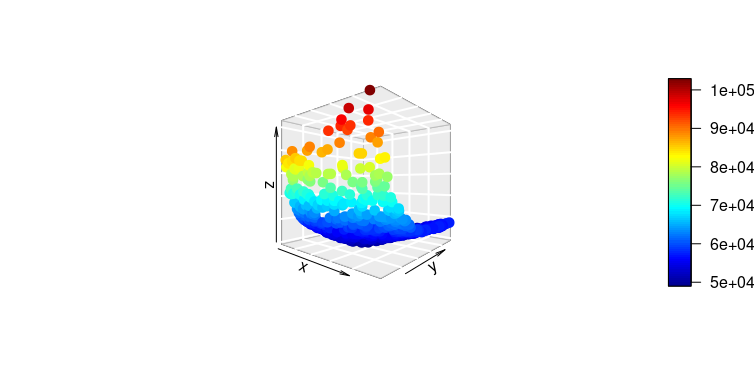
\includegraphics[width=0.3\linewidth]{Parameter Estimation on Attempt _1/param_1/lam0_5-0_75tau0-0_1.png}
            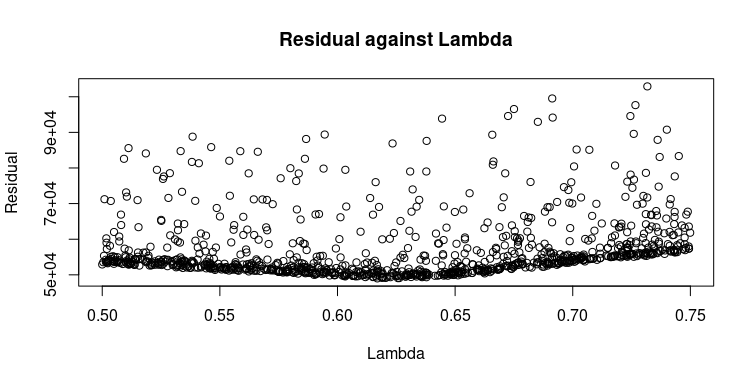
\includegraphics[width=0.3\linewidth]{Parameter Estimation on Attempt _1/param_1/lam_3.png}
            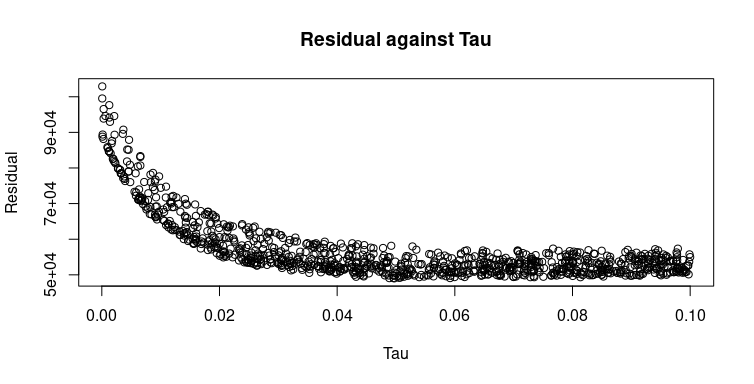
\includegraphics[width=0.3\linewidth]{Parameter Estimation on Attempt _1/param_1/tau_3.png}
        \end{columns}

    \end{frame}

    \section{Results and Future Research}
    \begin{frame}
        \frametitle{Results and Future Research}
        Kolmogorov–Smirnov tests

        \begin{itemize}
            \item \small{$H_0$: The two samples are from the same distribution}
            \item \small{$H_1$: The two samples are not from the same distribution.}
        \end{itemize}

        \begin{tabular}{c | c | c | c | c}
                &  Train & Train     & Test &  Test \\  
                \hline
            Month & HMM    & Gen Model & HMM  &  Gen Model\\
            \hline
            0     &   0.8593  &   \num{4.939e-5}     &   0.7899          &       \num{4.60e-08}   \\
            1     &   0.9969  &   0.002038          &   0.105           &        \num{5.46e-06}   \\
            2     &   1       &   \num{2.13e-05}     &   0.1118          &       \num{7.65e-07}   \\
            3     &   1       &   \num{1.79e-06}     &   0.02163         &       \num{1.11e-07}   \\
            4     &   0.4324  &   \num{1.38e-05}     &   0.0009582       &       \num{7.98e-08}   \\
            5     &   1       &   0.006202          &   0.2979          &       0.0004948  \\
            6     &   1       &   \num{1.11e-05}     &   0.1809          &       \num{8.53e-08}   \\
            7     &   1       &   \num{2.13e-05}     &   0.03555         &       \num{4.53e-05}   \\
            8     &   0.9999  &   0.0001108         &   0.07192         &       0.001033   \\
            9     &   0.9969  &   \num{6.06e-05}     &   \num{5.22e-07}   &       \num{1.22e-07}   \\
            10    &   0.8879  &   0.0008667         &   0.1914          &       \num{9.07e-05}   \\
            11    &   0.9999  &   \num{6.06e-05}     &   0.265           &       \num{2.15e-06}   
        \end{tabular}
        
    \end{frame}

\end{document}